\documentclass[12pt,t]{beamer}
\usepackage{graphicx}
\usepackage{tikz}
\setbeameroption{hide notes}
\setbeamertemplate{note page}[plain]
\usepackage{listings}

% header.tex: boring LaTeX/Beamer details + macros

% get rid of junk
\usetheme{default}
\beamertemplatenavigationsymbolsempty
\hypersetup{pdfpagemode=UseNone} % don't show bookmarks on initial view


% font
\usepackage{fontspec}
\setsansfont
  [ ExternalLocation = fonts/ ,
    UprightFont = *-regular ,
    BoldFont = *-bold ,
    ItalicFont = *-italic ,
    BoldItalicFont = *-bolditalic ]{texgyreheros}
\setbeamerfont{note page}{family*=pplx,size=\footnotesize} % Palatino for notes
% "TeX Gyre Heros can be used as a replacement for Helvetica"
% I've placed them in fonts/; alternatively you can install them
% permanently on your system as follows:
%     Download http://www.gust.org.pl/projects/e-foundry/tex-gyre/heros/qhv2.004otf.zip
%     In Unix, unzip it into ~/.fonts
%     In Mac, unzip it, double-click the .otf files, and install using "FontBook"

% named colors
\definecolor{offwhite}{RGB}{255,250,240}
\definecolor{gray}{RGB}{155,155,155}

\ifx\notescolors\undefined % slides
  \definecolor{foreground}{RGB}{255,255,255}
  \definecolor{background}{RGB}{24,24,24}
  \definecolor{title}{RGB}{107,174,214}
  \definecolor{subtitle}{RGB}{120,120,120}
  \definecolor{hilit}{RGB}{102,255,204}
  \definecolor{vhilit}{RGB}{255,111,207}
  \definecolor{codehilit}{RGB}{255,111,207}
  \definecolor{lolit}{RGB}{155,155,155}
\else % notes
  \definecolor{background}{RGB}{255,255,255}
  \definecolor{foreground}{RGB}{24,24,24}
  \definecolor{title}{RGB}{27,94,134}
  \definecolor{subtitle}{RGB}{120,120,120}
  \definecolor{hilit}{RGB}{122,0,128}
  \definecolor{vhilit}{RGB}{255,0,128}
  \definecolor{codehilit}{RGB}{24,24,24}
  \definecolor{lolit}{RGB}{95,95,95}
\fi
\definecolor{nhilit}{RGB}{128,0,128}  % hilit color in notes
\definecolor{nvhilit}{RGB}{255,0,128} % vhilit for notes

\newcommand{\hilit}{\color{hilit}}
\newcommand{\vhilit}{\color{vhilit}}
\newcommand{\nhilit}{\color{nhilit}}
\newcommand{\nvhilit}{\color{nvhilit}}
\newcommand{\lolit}{\color{lolit}}

% use those colors
\setbeamercolor{titlelike}{fg=title}
\setbeamercolor{subtitle}{fg=subtitle}
\setbeamercolor{institute}{fg=lolit}
\setbeamercolor{normal text}{fg=foreground,bg=background}
\setbeamercolor{item}{fg=foreground} % color of bullets
\setbeamercolor{subitem}{fg=lolit}
\setbeamercolor{itemize/enumerate subbody}{fg=lolit}
\setbeamertemplate{itemize subitem}{{\textendash}}
\setbeamerfont{itemize/enumerate subbody}{size=\footnotesize}
\setbeamerfont{itemize/enumerate subitem}{size=\footnotesize}

% page number
\setbeamertemplate{footline}{%
    \raisebox{5pt}{\makebox[\paperwidth]{\hfill\makebox[20pt]{\lolit
          \scriptsize\insertframenumber}}}\hspace*{5pt}}

% add a bit of space at the top of the notes page
\addtobeamertemplate{note page}{\setlength{\parskip}{12pt}}

% default link color
\hypersetup{colorlinks, urlcolor={hilit}}

\ifx\notescolors\undefined % slides
  % set up listing environment
  \lstset{language=bash,
          basicstyle=\ttfamily\scriptsize,
          frame=single,
          commentstyle=,
          backgroundcolor=\color{darkgray},
          showspaces=false,
          showstringspaces=false
          }
\else % notes
  \lstset{language=bash,
          basicstyle=\ttfamily\scriptsize,
          frame=single,
          commentstyle=,
          backgroundcolor=\color{offwhite},
          showspaces=false,
          showstringspaces=false
          }
\fi

% a few macros
\newcommand{\bi}{\begin{itemize}}
\newcommand{\bbi}{\vspace{24pt} \begin{itemize} \itemsep8pt}
\newcommand{\ei}{\end{itemize}}
\newcommand{\ig}{\includegraphics}
\newcommand{\subt}[1]{{\footnotesize \color{subtitle} {#1}}}
\newcommand{\ttsm}{\tt \small}
\newcommand{\ttfn}{\tt \footnotesize}
\newcommand{\figh}[2]{\centerline{\includegraphics[height=#2\textheight]{#1}}}
\newcommand{\figw}[2]{\centerline{\includegraphics[width=#2\textwidth]{#1}}}


%%%%%%%%%%%%%%%%%%%%%%%%%%%%%%%%%%%%%%%%%%%%%%%%%%%%%%%%%%%%%%%%%%%%%%
% end of header
%%%%%%%%%%%%%%%%%%%%%%%%%%%%%%%%%%%%%%%%%%%%%%%%%%%%%%%%%%%%%%%%%%%%%%

% title info

\title{Automating Reproducibility}
\subtitle{A Reproducible Data Analysis Workflow with R\nobreakspace{}Markdown, Git, Make, and Docker}
\author{\href{https://github.com/aaronpeikert/}{Aaron Peikert\textsuperscript{1,2}\\ \&\\ Andreas Brandmaier\textsuperscript{1}}}
\institute{
\textsuperscript{1}Max Planck Institute of Human Development\\
\textsuperscript{2}Humboldt{\textendash}Universität zu Berlin
}
\date{
\scriptsize {\lolit Slides:} \href{https://github.com/aaronpeikert/repro-talk}{\tt \scriptsize
  \color{foreground} https://github.com/aaronpeikert/repro-talk}
}


\begin{document}

% title slide
{
{
\setbeamertemplate{footline}{} % no page number here
\frame{
  \titlepage

  \vfill \hfill 
\includegraphics[height=6mm]{Figs/cc-zero.png} \vspace*{-1cm}

  \note{These Slides are for a medium length talk (30min) meant as an introduction to a reproducible research workflow.

    Source: {\tt https://github.com/aaronpeikert/repro-talk}
}}
}
\begin{frame}[c]
  \begin{center}
  \large
  \textcolor<2>{lolit}{``Insanity is doing the same thing over and over again and expecting different results."}
  \end{center}
  \textcolor<2>{lolit}{\hfill {\textendash} Albert Einstein}\\
  \onslide<2>{
  \begin{center}
  As it turns out doing the\\
    \textcolor{hilit}{{\large same thing}}\\
  is pretty complicated.
\end{center}}

\end{frame}
\begin{frame}[c]{Reproduction ≠ Replication}
  If everything is allready there:
\begin{itemize}
  \item published paper
  \item data originally used
  \item code originally used
\end{itemize}
\onslide<2->{Shouldn't that be enough? }\onslide<3>{\textcolor{hilit}{Unlikely.}}
\end{frame}

{
  \usebackgroundtemplate{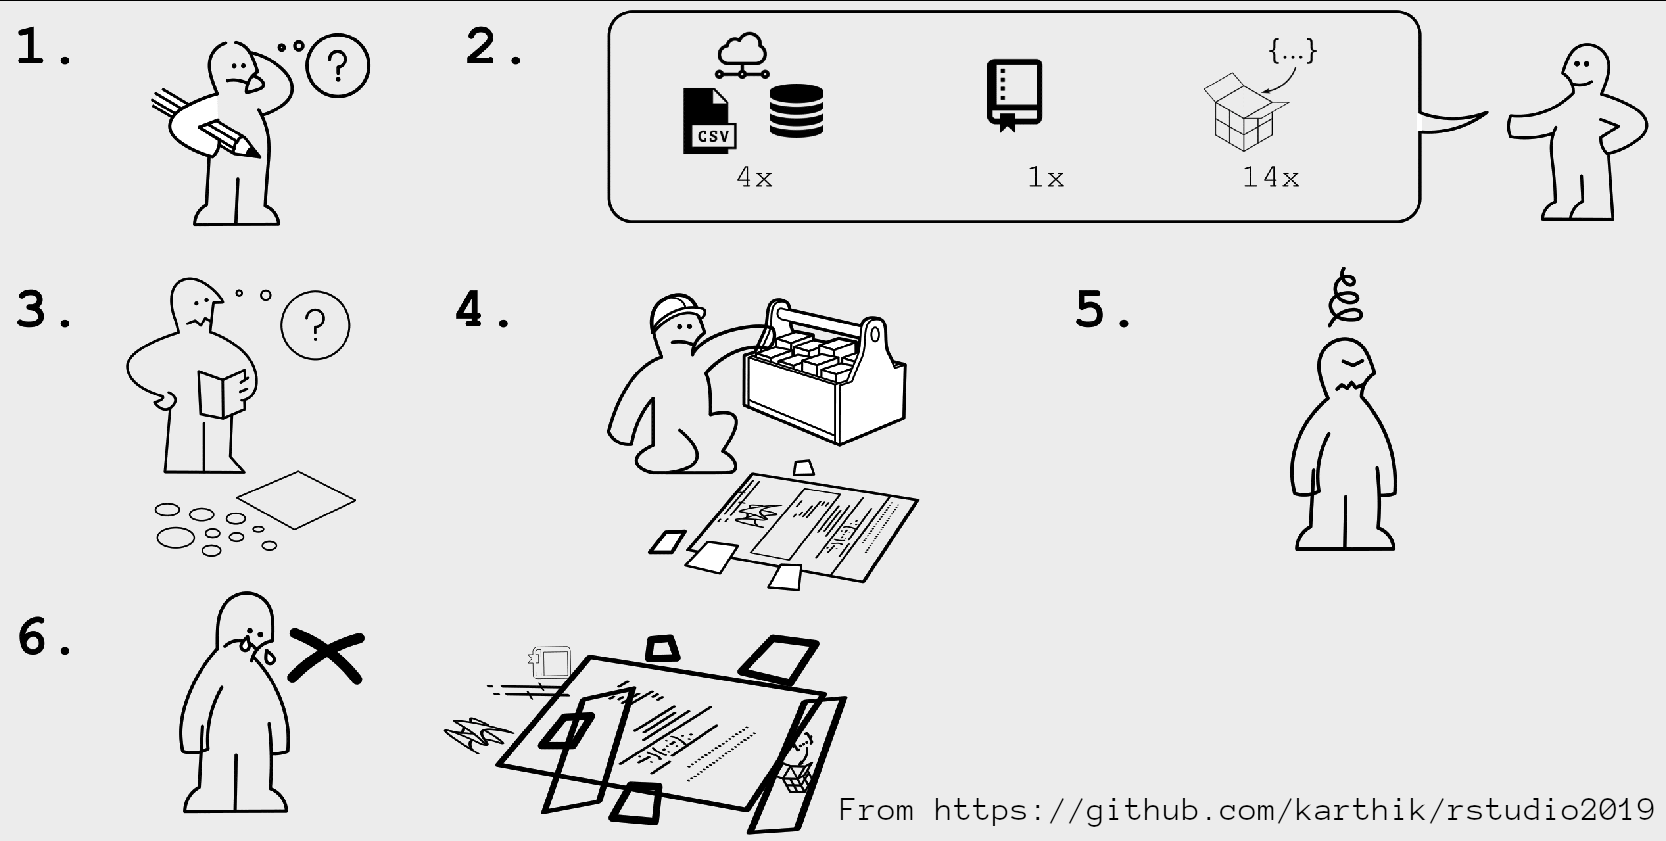
\includegraphics[width=\paperwidth]{Figs/ikea.png}}
  \begin{frame}[plain]
  \end{frame}
}

\begin{frame}[c]{Specify Everything}
  \textcolor<3->{lolit}{The relations between\\
  \textcolor<2>{hilit}{code}, \textcolor<2>{hilit}{data}, \textcolor<2>{hilit}{results} and their \textcolor<2>{hilit}{environment}\\
  need to be \textcolor<2>{vhilit}{unambiguously} specified.\\}
  \vspace{10mm}
  \onslide<3->{\textcolor<4->{lolit}{
  IMHO: Only computer code is unambiguous.\\}}
  \onslide<4>{Spoiler: Computer code is \textcolor{hilit}{not} unambiguous.}
\end{frame}

\begin{frame}[c]{Concepts to fix relations}
  \begin{itemize}
    \item Code \textemdash{} document = literate programming
    \item Code version \textemdash{} data version = version control
    \item Code \textemdash{} interim results = dependency management
    \item Code \textemdash{} execution environment = containerization
  \end{itemize}
\end{frame}

\begin{frame}[c]{Tools for R Users}
  \begin{itemize}
    \item literate programming = RMarkdown
    \item version control = Git
    \item dependency management = Make
    \item containerization = Docker
  \end{itemize}
  \vfill
  \textcolor{lolit}{*Note: There are many great alternatives,\\they just happen to be not used as much.}
\end{frame}

\begin{frame}[c]{RMarkdown\textemdash{}Literate Programming}
  Text and code are intermingled\\
  into a single source document\\
  that can be dynamically compiled\\
  into varius representations:
  \begin{itemize}
    \item (apa conformable) manuscripts
    \item presentations
    \item websites
    \item books
    \item posters
  \end{itemize}
\end{frame}

{
  \usebackgroundtemplate{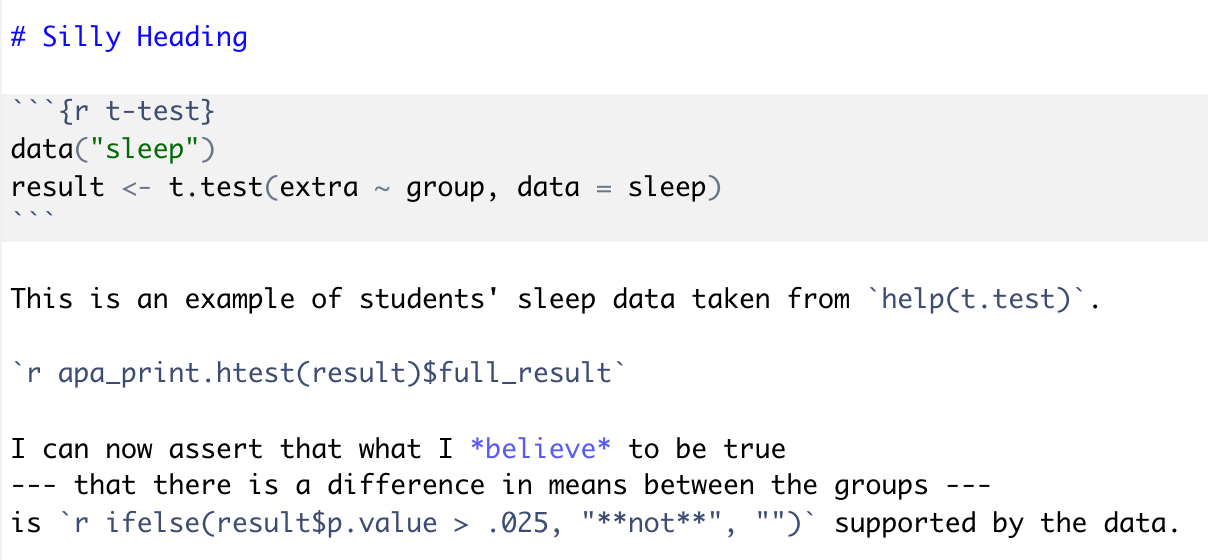
\includegraphics[width=\paperwidth]{Figs/rmarkdown.png}}
  \begin{frame}[plain]
  \end{frame}
}
{
  \usebackgroundtemplate{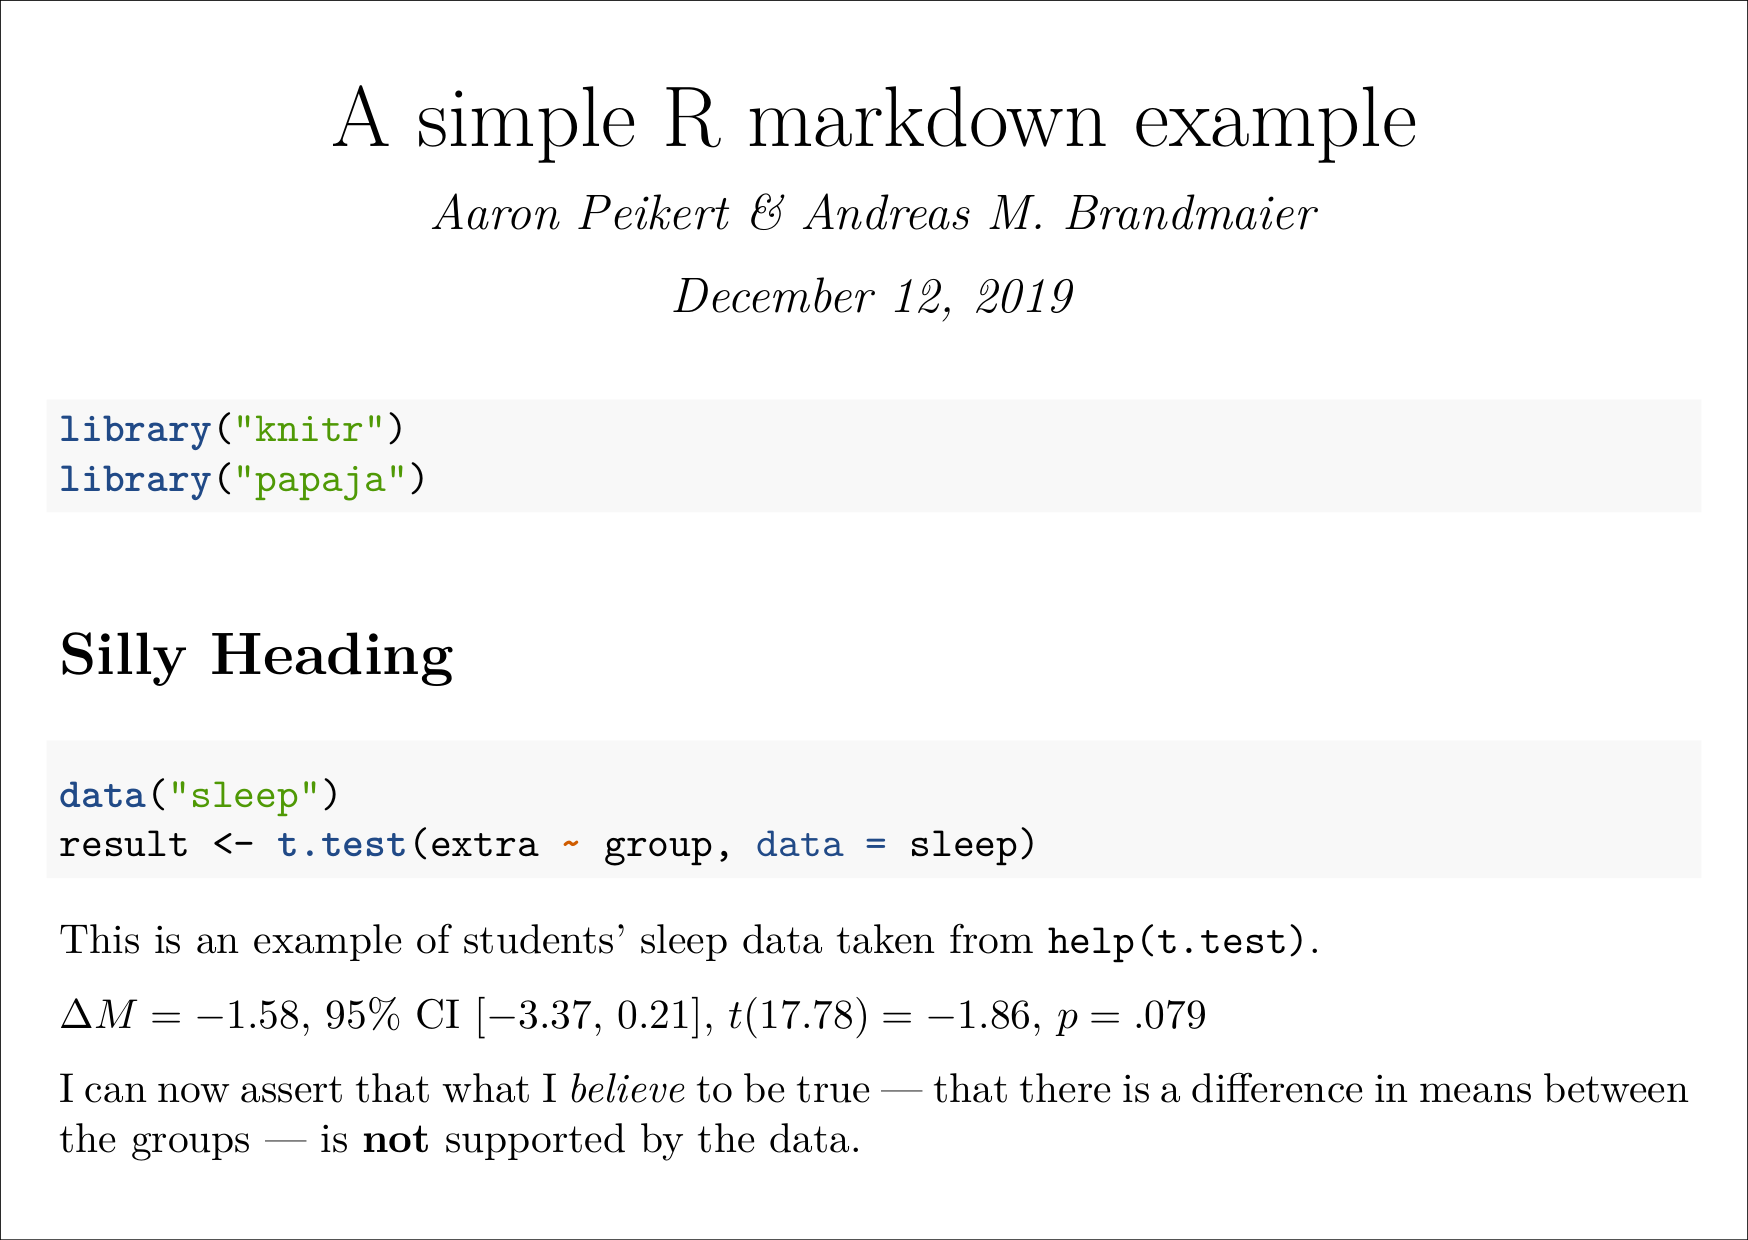
\includegraphics[width=\paperwidth]{Figs/rmarkdown-rendered.png}}
  \begin{frame}[plain]
  \end{frame}
}
\begin{frame}[c]{Git/GitHub\textemdash{}Version Control}
  Version control is a system that records changes to set of files
  over time so that you can recall specific versions later.\\
  \vspace{10mm}
  It guarantees that code and data are exactly the same version as used for
  publication.
\end{frame}
\begin{frame}[c]{Make\textemdash{}Dependency Management}

I would argue that the most important tool for reproducible research is [...] GNU make.\\
\hfill {\textendash} \href{https://kbroman.org/minimal_make/}{Karl Broman}\\

\end{frame}

\begin{frame}[c, fragile]{Make\textemdash{}Dependency Management}

Make is ``recipe" language that describes how files relate to each other.
\vspace{10mm}
\begin{lstlisting}[language=make,basicstyle=\ttfamily\scriptsize]
cfcs-example.pdf: cfcs-example.Rmd data/CFCS.csv
  $(run) Rscript -e 'rmarkdown::render("$(current_dir)/$<")'

data/CFCS.csv: R/00load_data.R
  $(run) Rscript -e 'source("$(current_dir)/$<")'
\end{lstlisting}
\end{frame}

\begin{frame}[c, fragile]{Docker\textemdash{}Containerization}
	Docker is a lightweight virtual computer that is completly independant.\\
	Dockerfiles are ``recipies" which describe what to install on that virtual computer:
	\vspace{10mm}
	\begin{lstlisting}[language=make,basicstyle=\ttfamily\scriptsize]
FROM rocker/verse:3.6.1
ARG BUILD_DATE=2019-11-11
RUN install2.r --error --skipinstalled\
  here lavaan
WORKDIR /home/rstudio
\end{lstlisting}
\end{frame}

\begin{frame}[c]{Future}

\begin{itemize}
	\item The `repro' package shall:
	\begin{itemize}
		\item ease the instalation process
		\item automatize the setup of new projects
		\item abstract away Docker \& Make
		\item enable automatic execution on GitHub
	\end{itemize}
	\item hands on workshop
	\begin{itemize}
		\item Where? MPI Berlin.
		\item When? 20.02.20 10-16
	\end{itemize}
	\item \textcolor{lolit}{replicable preregistered collaboration project}
\end{itemize}
\vspace{10mm}
Interested?! Write me an e-mail:\\ \hfill \textcolor{lolit}{peikert@mpib-berlin.mpg.de}
\end{frame}

\end{document}
